\chapter{Proximal Optimization for Boolean Matrix Factorization}
\label{chap:PALMB}
In a large range of exploratory data mining tasks such as Market Basket Analysis, Text Mining, Collaborative Filtering or DNA Expression Analysis, the data is represented by a binary matrix. In this case, a binary representation of the cluster centers is desirable to reflect the binary nature of features. Methods which provide interpretable models in that sense are discussed from the viewpoint of binary matrix factorization, pattern mining, tiling and Boolean matrix factorization~\citep{tatti2012comparing,zimek2015blind}. Of those fields, Boolean matrix factorization is the most flexible one. Boolean factorizations are not required to model partitioning cluster assignments, such as binary matrix factorization and it does not restrict the cluster assignment to the support of a pattern, as is the case in tiling and pattern mining. 
 
Therefore, providing a generic optimization method, solving the problem of~\ref{eq:BoolMF}, has a possible impact on the optimization of all the regarded cluster objectives in Chapter~\ref{chap:ZeroShades}. We have seen that the optimization of non-partitioning clusters is by and large an unsolved problem. Approaches tackling this issue require detailed specifications of parameters which are unknown in advance, such as the amount of overlap and outliers~\citep{whang2017nonCo}. In contrast, we aim at formalizing an optimization scheme which is able to derive the \emph{true} model, regardless of the characteristics of that model; may it be overlapping or not, may it have a large amount of overlap or not. 

%------------FIGURE INTRO SPACE INVADERS-----------
\begin{figure}
  \begin{align*}
      \vcenter{\hbox{
\includegraphics[scale =0.2]{pics/SpaceInv/spaceInv}}} 
      &\approx
      \vcenter{\hbox{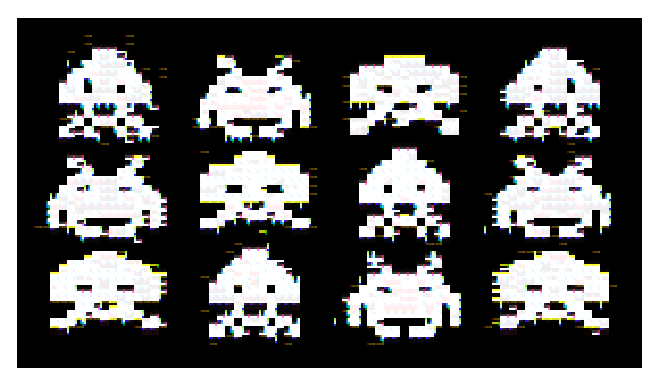
\includegraphics[scale =0.2]{pics/SpaceInv/PandaspaceInv}}}
      = \vcenter{\hbox{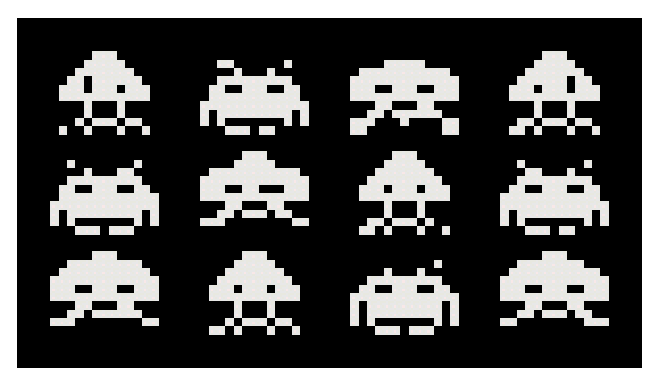
\includegraphics[scale =0.2]{pics/SpaceInv/PandaspaceInv1}}}
     \oplus \vcenter{\hbox{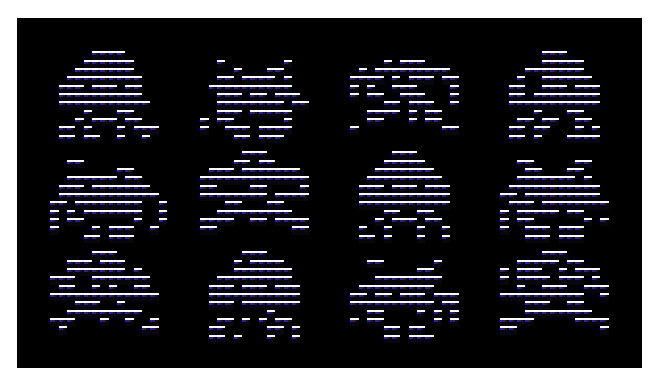
\includegraphics[scale =0.2]{pics/SpaceInv/PandaspaceInv2}}}
     \oplus \vcenter{\hbox{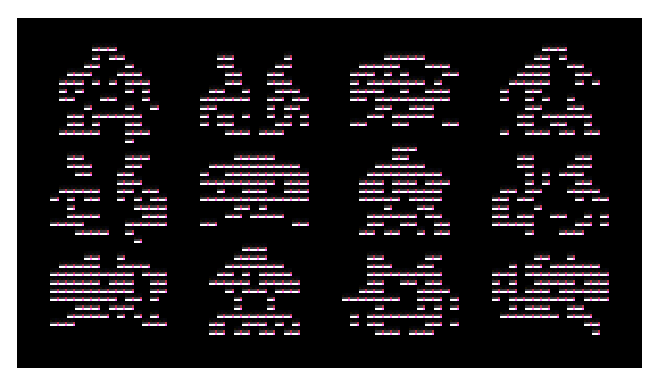
\includegraphics[scale =0.2]{pics/SpaceInv/PandaspaceInv3}}}\\
     \vcenter{\hbox{
\includegraphics[scale =0.2]{pics/SpaceInv/spaceInv}}}
     &\approx
     \vcenter{\hbox{
\includegraphics[scale =0.2]{pics/SpaceInv/PrimpSpaceInv}}}
    = \vcenter{\hbox{
\includegraphics[scale =0.2]{pics/SpaceInv/PrimpSpaceInv1}}}
    \oplus \vcenter{\hbox{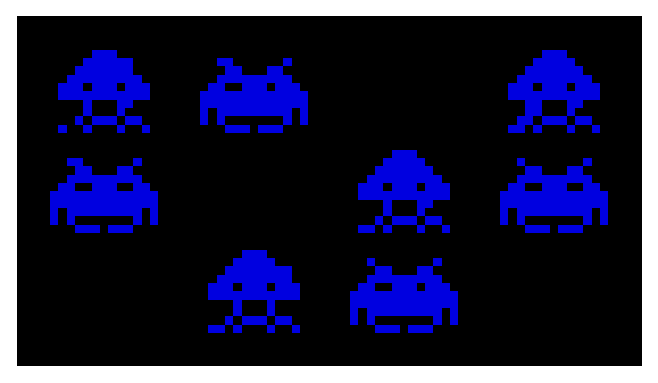
\includegraphics[scale =0.2]{pics/SpaceInv/PrimpSpaceInv2}}}
    \oplus \vcenter{\hbox{
\includegraphics[scale =0.2]{pics/SpaceInv/PrimpSpaceInv3}}}
  \end{align*}
  \caption{Results of a Boolean decomposition of rank three on a picture dataset, depicted on the left. On the top row, the picture is approximated by a greedy approach, on the bottom we display the result of the proposed proximal optimization scheme for BMF. Best viewed in color.\label{fig:PT:introSpaceInv}}
\end{figure}
Unfortunately, present \ref{eq:BoolMF} optimizations employ a greedy heuristic, which can not provide guarantees as known from numerical optimization methods, such as convergence to a local optimum. We make use of an example to show the innate disadvantage, emerging from a strong preference bias of the greedy approach in Figure~\ref{fig:PT:introSpaceInv}. Here, a picture is transformed into a binary data matrix via its binary representation in RGB888 pixel format. On the top row, you see the decomposition obtained by the greedy approach \textsc{Panda+}~\citep{lucchese2014unifying} and on the bottom the approximation derived by the new method which we introduce in this chapter. Each of the three rightmost pictures visualizes an outer product, also called tile in the context of binary factorization. The difference between both results is striking, in particular because the color information gets completely lost in the greedy approximation. We observe that the greedy representation in black and white is attributed to the first outer product being overloaded with the information about shape. Since the color white has a binary representation as a constant one vector, any white pixel in one outer product picture also appears white in the resulting approximation. Accordingly, the greedy approach is very sensitive to making mistakes in the first derived tiles and is therewith also susceptible to noise. In contrast, we propose a simultaneous optimization of the clusters based on a nonnegative relaxation with binary penalization. This approach is similar to the binary factorization by~\cite{zhang2007binary}, employing the mexican hat function for the penalization of nonbinary values (cf.\@ Section~\ref{sec:ZS:Penalty}). However, our method follows latest results in nonconvex optimization theory and provides a general framework for the efficient optimization of matrix factorization under binary constraints. The main contribution of this chapter is the derivation of the proximal mapping, which implements the nonbinary penalization. This proximal mapping is usable as a building block to incorporate binary restrictions on one of the matrices in factorization objectives. Known proximal mappings involving other constraints such as nonnegativity, sparseness or the restriction to the probability simplex can then be integrated within the larger optimization framework.  

%=================================================
% Approximating the Boolean Product in Elementary Algebra
%=================================================
\section{Approximating the Boolean Product in Elementary Algebra}
A possible reason for the prevailing usage of heuristics in Boolean matrix factorization is the reasonable belief that relaxations to nonnegative or other  continuous values are not apt to approximate a product in Boolean arithmetic. Contrary to this belief, we argue for the opposite; a nonnegative relaxation is particularly suited to derive overlapping clusterings and is therefore also suited to approximate Boolean matrix factorizations, whose main characteristic is to allow for overlap between the clusters. Now we need to be a bit careful with the word \emph{approximate}. The \ref{eq:BoolMF} problem is NP-hard and NP-hard to aproximate within a constant factor~\citep{miettinen2008discrete}. Hence, we will not be able to produce an efficient algorithm which comes arbitrarily close to the optimal Boolean solution (unless NP=P). Yet we are able to simulate some of the required characteristics of Boolean solutions in a relaxed space. 

%--------- FIGURE OVERLAPPING FACTORIZATION ------------
\begin{figure}
\centering
\begin{align*}
D=
\begin{tikzpicture}[baseline=-0.5ex]
   \matrix [matrix of math nodes,left delimiter=(,right delimiter=),ampersand replacement=\&] (n) {
1\&1\&1\&0 \\
1\&1\&1\&1 \\
0\&1\&1\&1 \\
};
\draw[color=col1,fill=col1,opacity=0.2] (n-1-1.north west) -- (n-1-3.north east) -- (n-2-3.south east) -- (n-2-1.south west) -- (n-1-1.north west);
\draw[color=col2,fill=col2,opacity=0.2] (n-2-2.north west) -- (n-2-4.north east) -- (n-3-4.south east) -- (n-3-2.south west) --(n-2-2.north west);
\end{tikzpicture}
&\approx
%----------------------------
%\\
%----------------------------
\begin{tikzpicture}[baseline=-0.5ex]
   \matrix [matrix of math nodes,left delimiter=(,right delimiter=),ampersand replacement=\&] (n) {
\phantom{.}1\&\phantom{1}.9\&\phantom{1}.9\&.1 \\
.7\&1.2\&1.2\&.7 \\
.1\&\phantom{1}.9\&\phantom{1}.9\&1\phantom{.} \\
};
\draw[color=col1,fill=col1,opacity=0.2] (n-1-1.north west) -- (n-1-3.north east) -- (n-2-3.south east) -- (n-2-1.south west) -- (n-1-1.north west);
\draw[color=col2,fill=col2,opacity=0.2] (n-2-2.north west) -- (n-2-4.north east) -- (n-3-4.south east) -- (n-3-2.south west) --(n-2-2.north west);
\end{tikzpicture}
%---------------------
\\
%---------------------
&\approx
\begin{tikzpicture}[baseline=-0.5ex]
    \matrix [matrix of math nodes,left delimiter=(,right delimiter=),ampersand replacement=\&] (n) {
1\phantom{.}\&0 \\
.6\&.6 \\
0\&1\phantom{.} \\
};
\draw[color=col1,fill=col1,opacity=0.2] (n-1-1.north west) -- (n-1-1.north east) -- (n-2-1.south east) -- (n-2-1.south west) -- (n-1-1.north west);
\draw[color=col2,fill=col2,opacity=0.2] (n-2-2.north west) -- (n-2-2.north east) -- (n-3-2.south east) -- (n-3-2.south west) --(n-2-2.north west);
\end{tikzpicture}
\cdot
\begin{tikzpicture}[baseline=-0.5ex]
    \matrix [matrix of math nodes,left delimiter=(,right delimiter=),ampersand replacement=\&] (n) {
1\&.9\&.9\&.1 \\
.1\&.9\&.9\&1 \\
};
\draw[color=col1,fill=col1,opacity=0.2] (n-1-1.north west) -- (n-1-3.north east) -- (n-1-3.south east) -- (n-1-1.south west) --(n-1-1.north west);
\draw[color=col2,fill=col2,opacity=0.2] (n-2-2.north west) -- (n-2-4.north east) -- (n-2-4.south east) -- (n-2-2.south west) -- (n-2-2.north west);
\end{tikzpicture}
%-------------------------------------
\\
%-----------------------------
D_A=
\begin{tikzpicture}[baseline=-0.5ex]
   \matrix [matrix of math nodes,left delimiter=(,right delimiter=),ampersand replacement=\&] (n) {
1\&1\&1\&0 \\
1\&2\&2\&1 \\
0\&1\&1\&1 \\
};
\draw[color=col1,fill=col1,opacity=0.2] (n-1-1.north west) -- (n-1-3.north east) -- (n-2-3.south east) -- (n-2-1.south west) -- (n-1-1.north west);
\draw[color=col2,fill=col2,opacity=0.2] (n-2-2.north west) -- (n-2-4.north east) -- (n-3-4.south east) -- (n-3-2.south west) --(n-2-2.north west);
\end{tikzpicture}
&=
\mathlarger{\theta}
\begin{tikzpicture}[baseline=-0.5ex]
    \matrix [matrix of math nodes,left delimiter=(,right delimiter=),ampersand replacement=\&] (n) {
1\phantom{.}\&0 \\
.6\&.6 \\
0\&1\phantom{.} \\
};
\draw[color=col1,fill=col1,opacity=0.2] (n-1-1.north west) -- (n-1-1.north east) -- (n-2-1.south east) -- (n-2-1.south west) -- (n-1-1.north west);
\draw[color=col2,fill=col2,opacity=0.2] (n-2-2.north west) -- (n-2-2.north east) -- (n-3-2.south east) -- (n-3-2.south west) --(n-2-2.north west);
\end{tikzpicture}
\cdot \mathlarger{\theta}
\begin{tikzpicture}[baseline=-0.5ex]
    \matrix [matrix of math nodes,left delimiter=(,right delimiter=),ampersand replacement=\&] (n) {
1\&.9\&.9\&.1 \\
.1\&.9\&.9\&1 \\
};
\draw[color=col1,fill=col1,opacity=0.2] (n-1-1.north west) -- (n-1-3.north east) -- (n-1-3.south east) -- (n-1-1.south west) --(n-1-1.north west);
\draw[color=col2,fill=col2,opacity=0.2] (n-2-2.north west) -- (n-2-4.north east) -- (n-2-4.south east) -- (n-2-2.south west) -- (n-2-2.north west);
\end{tikzpicture}
%------------------------------
\\
%------------------------------
D_B=
\begin{tikzpicture}[baseline=-0.5ex]
   \matrix [matrix of math nodes,left delimiter=(,right delimiter=),ampersand replacement=\&] (n) {
1\&1\&1\&0 \\
1\&1\&1\&1 \\
0\&1\&1\&1 \\
};
\draw[color=col1,fill=col1,opacity=0.2] (n-1-1.north west) -- (n-1-3.north east) -- (n-2-3.south east) -- (n-2-1.south west) -- (n-1-1.north west);
\draw[color=col2,fill=col2,opacity=0.2] (n-2-2.north west) -- (n-2-4.north east) -- (n-3-4.south east) -- (n-3-2.south west) --(n-2-2.north west);
\end{tikzpicture}
&=
\mathlarger{\theta}\left(\mathlarger{\theta}
\begin{tikzpicture}[baseline=-0.5ex]
    \matrix [matrix of math nodes,left delimiter=(,right delimiter=),ampersand replacement=\&] (n) {
1\phantom{.}\&0 \\
.6\&.6 \\
0\&1\phantom{.} \\
};
\draw[color=col1,fill=col1,opacity=0.2] (n-1-1.north west) -- (n-1-1.north east) -- (n-2-1.south east) -- (n-2-1.south west) -- (n-1-1.north west);
\draw[color=col2,fill=col2,opacity=0.2] (n-2-2.north west) -- (n-2-2.north east) -- (n-3-2.south east) -- (n-3-2.south west) --(n-2-2.north west);
\end{tikzpicture}
\cdot \mathlarger{\theta}
\begin{tikzpicture}[baseline=-0.5ex]
    \matrix [matrix of math nodes,left delimiter=(,right delimiter=),ampersand replacement=\&] (n) {
1\&.9\&.9\&.1 \\
.1\&.9\&.9\&1 \\
};
\draw[color=col1,fill=col1,opacity=0.2] (n-1-1.north west) -- (n-1-3.north east) -- (n-1-3.south east) -- (n-1-1.south west) --(n-1-1.north west);
\draw[color=col2,fill=col2,opacity=0.2] (n-2-2.north west) -- (n-2-4.north east) -- (n-2-4.south east) -- (n-2-2.south west) -- (n-2-2.north west);
\end{tikzpicture}
\right)
\end{align*}
\caption{Approximation of a binary matrix $D$ with two overlapping tiles (top) applying NMF (second from above) and the factorizations resulting from thresholding the factor matrices to binary matrices in elementary algebra (second from below) and Boolean algebra (below). Tiles are highlighted.}
\label{fig:overlapFact}
\end{figure}
%-------------------------------------------------------
To make our case, we inspect how nonnegative and Boolean matrix factorizations deal with overlapping clusters. An example binary data matrix consisting of two  overlapping tiles and its approximation by a nonnegative matrix factorization is shown in the top two equations of Figure~\ref{fig:overlapFact}. We see that the factors contain values smaller than one at entries which are involved in overlapping parts. With this, overlapping sections are equally well approximated as non-overlapping components. 
The matrices $D_A$ and $D_B$ in Figure~\ref{fig:overlapFact} show the resulting binary and Boolean approximations, thresholding the nonnegative factor matrices at one half. We find that the reconstruction error is largest when the thresholded matrices are multiplied in elementary algebra, as it is the case in binary matrix factorization. In contrast, the fuzzy cluster indication by NMF is suited to indicate a definite clustering with respect to the Boolean algebra. This seems at first contradictory to the discussed near-orthogonality of NMF solutions in Section~\ref{sec:ZS:NMFClus}. However, although NMF has an in-built penalization of nonorthogonal factor matrices (cf.\@ Eq.~\eqref{eq:NMFOrth}), the approximation error is the dominating value of the objective function. Accordingly, the better the factorization approximates the data, implying the higher the rank, the more become solutions of \ref{eq:NMF} orthogonal. Conversely, we conclude that overlap between clusters is mirrored by a nonnegative approximation if the rank is low.   
%==================================
% Proximal Alternating Linearized Minimization
%==================================
\section{Proximal Alternating Linearized Minimization}
Standard gradient descent-based optimization schemes for~\ref{eq:NMF} problems are either multiplicative updates or projected gradient methods. The crucial aspect of both optimization schemes is the determination of the stepsize. The optimization with multiplicative updates is slow due to the conservative choice  of the stepsize, ensuring that factor matrices are nonnegative. Projected gradient methods often employ a linesearch procedure to determine the optimal stepsize, but calculating the optimal stepsize in every step is also costly.

\cite{bolte2014proximal} extend optimization results known for convex optimization to the nonconvex case with the \emph{Proximal Alternating Linearized Minimization} (PALM). This technique focuses on objectives breaking down into a smooth part $F$ and a possibly nonsmooth component $\phi$
\begin{align}\label{eq:PalmObj}
 \min_{X,Y}&\	F(X,Y)+ \phi_1(X) +\phi_2(Y) &\text{s.t. }X\in\mathbb{R}^{n\times r}, Y\in\mathbb{R}^{m\times r}.
\end{align}
The function $F$ reflects here the objective function or its smooth relaxation. We assume for now that $F(X,Y)=\bigl\lVert D-YX^\top\bigr\rVert ^2$ returns the approximation error in the Frobenius norm. 
The nonsmooth part $\phi$ may return $\infty$, which can be used to model restrictions of the search space, e.g., the nonnegativity constraint of NMF. 
PALM performes an alternating minimization on the linearized objective, substituting $F$ with its first order Taylor approximation. This is achieved by alternating \emph{proximal mappings} from the gradient descent update with respect to $F$, i.e., the following steps are repeated for $1\leq k \leq K$:
\begin{align}\label{eq:PalmIterX}
X_{k+1} &= \prox_{\alpha_k\phi_1}(X_k-\alpha_k\nabla_XF(X_k,Y_k));\\
Y_{k+1} &= \prox_{\beta_k\phi_2}(Y_k-\beta_k\nabla_YF(X_{k+1},Y_k)).\label{eq:PalmIterY}
\end{align}
The proximal mapping of a function $\phi$, is a function which returns a matrix satisfying the following minimization criterion: 
\begin{align}\label{eq:prox}
    \prox_\phi(X) \in \argmin_{X^*}\left\{\frac{1}{2}\lVert X-X^*\rVert ^2+\phi(X^*)\right\}.
\end{align}
Loosely speaking, the proximal mapping gives its argument a little push into a direction which minimizes $\phi$. For a detailed discussion, see, e.g., \citep{parikh2014proximal}. As we can see in Eqs.~(\ref{eq:PalmIterX}) and (\ref{eq:PalmIterY}), the evaluation of this operator is a base operation. Similarly to the alternating minimization in Eq.~(\ref{eq:als}), finding the minimum of the proximal mapping in every iteration by numerical methods is infeasible in practice. Thus, the trick is to use only simple functions $\phi$ for which the proximal mapping can be calculated in a closed form. 

%------------------------------
% Convergence Results
%-------------------------------
\subsection{Convergence Results}
We state here the main convergence result for PALM in a specified version, requiring that the differentiable part of the objective is smooth and not only continuously differentiable, summarizing the discussion with respect to smooth functions in \citep{bolte2014proximal}. Yet first, we need to introduce some definitions.
\begin{definition}[proper, semi-continuous function] Let $f:\mathbb{R}^{n}\rightarrow (-\infty,\infty]$ be an extended real-valued function. We say $f$ is \emph{proper} if there exists at least one $x\in\mathbb{R}^n$ such that $f(x)<\infty$. The function $f$ is called \emph{lower semi-continuous} if for all $x_0\in\mathbb{R}^n$ the
\[\liminf_{x\rightarrow x_0}f(x)\geq f(x_0).\]
\end{definition}
%------------FIGURE LOWER SEMI-Continuous-----
\begin{figure}
\centering
\begin{tikzpicture}%[scale =0.8]
	\begin{axis}[width=200pt,height = 90pt, axis x line=left, domain=-1:4,ymin=-0.2, axis y line=center, tick align=outside,legend pos=outer north east,legend style={cells={align=left,anchor=west}}]
    	\addplot+[domain=-1:1,mark=none,smooth,col1,ultra thick,samples=100] (\x,\x^2);
    	\addplot+[domain=1:3,mark=none,smooth,col1,ultra thick,samples=100] (\x,{-4*(\x-1.5)^2+4});
        \draw [draw=col1, fill=col1, ultra thick] 
            (axis cs: 1, 1) circle (2.0pt);
    	\draw [draw=col1, fill=white, ultra thick] 
            (axis cs: 1, 3) circle (2.0pt);	
        \addlegendentry{$f(x)=\begin{cases}x^2 & x\leq 1\\ -4(x-1.5)^2+4 & x>1 \end{cases}$\\};
	\end{axis}
\end{tikzpicture}
\caption{A lower semi-continuous function.}
\label{fig:PT:lowerSemiCont}
\end{figure}
The convergence analysis of PALM requires that the nonsmooth part $\phi$ is a proper, lower semi-continuous function. In practice, this is not a demanding requirement.
We display an example of a lower semi-continuous function in Figure~\ref{fig:PT:lowerSemiCont}. Let us exercise what is stated in the definition by this example. The function $f$ has a point of discontinuity at $x=1$. Any limit point of function values $f(x_k)$ for a sequence converging to the point of discontinuity ($x_k\rightarrow 1$) is either equal to one or to three. Thus, we have $\{1,3\}\ni\liminf_{x\rightarrow 1}f(x)\geq f(1)=1$. In other words, lower semi-continuous functions always attain the lowest limit point of function values. The restriction to lower semi-continuous functions $\phi$ ensures inter alia that the prox-operator is well-defined (cf.\@ Eq.~\eqref{eq:prox}).
%-----------
\begin{definition}[Kurdyka-Lojasiewicz functions]
Let $f:\mathbb{R}^{n}\rightarrow \mathbb{R}\cup\{\infty\}$ be a proper lower semi-continuous function and $x_0\in\mathbb{R}^n$, such that\footnote{$\partial $ denotes here the Fr\'{e}chet subdifferential} $\partial f(x_0)\neq\emptyset$. Define a subset of real-valued, continuous functions as
\[\mathcal{K}=\{\kappa:[0,t)\rightarrow \mathbb{R}_+\mid t\in(0,\infty],\kappa(0)=0,\kappa\in C^1(0,t), \kappa\in C^0[0,t)\}.\] 
The function $f$ is said to have the \emph{Kurdyka-{\L}ojasiewicz property} at point $x_0$ if there exists a concave and strictly increasing function $\kappa\in\mathcal{K}$ and an $\epsilon>0$ such that for all 
$x\in \mathcal{N}_\epsilon(x_0)$ satisfying $f(x_0)<f(x)<f(x_0)+t$
the Kurdyka-{\L}ojasiewicz inequality holds for all vectors $g\in\partial f(x)$, that is
\[\kappa^\prime\left(f(x)-f(x_0)\right)\lVert g\rVert \geq 1.\]
A function $f$ is called Kurdyka-{\L}ojasiewicz function if it has the Kurdyka-{\L}ojasiewicz property at any point $x_0$ where $\emptyset \neq \partial f$. 
\end{definition}
The impact that a requirement of the Kurdyka-{\L}ojasiewicz property has is not easy to understand. Here, it is only important to know which class of functions satisfy this property and how we can derive for specified functions if they satisfy the Kurdyka-{\L}ojasiewicz property. For this reason, we state some of the general rules from which we can conclude the \KL property for a given function in the following section. The following theorem states the main convergence result for PALM.

\begin{theorem}{{\citep{bolte2014proximal}}}\label{thm:palmConv}
Let $F:\mathbbm{R}^{n\times r}\times \mathbbm{R}^{m\times r}\rightarrow \mathbbm{R}_+$ be a smooth function and let $\phi_1:\mathbbm{R}^{n\times r}\rightarrow [0,\infty]$ and $\phi_2:\mathbbm{R}^{m\times r}\rightarrow [0,\infty]$ be proper and lower semi-continuous functions. Denote with $(\mathcal{X},\mathcal{Y})\subseteq\mathbb{R}^{n\times r}\times \mathbbm{R}^{m\times r}$ the feasible set, defined as
\begin{align*}
    \mathcal{X} = \{X\in \mathbb{R}^{n\times r}\mid \phi_1(X)<\infty\}\quad \text{and} \quad \mathcal{Y} = \{Y\in \mathbb{R}^{m\times r}\mid \phi_2(Y)<\infty\},
\end{align*}
Assume that the following conditions hold:
\begin{enumerate}
\item the partial gradients of $F$ are Lipschitz-continuous, satisfying the following inequality for real-valued functions $M_{\nabla_XF}(Y)$ and $M_{\nabla_YF}(X)$
\begin{align*}
\lVert \nabla_XF(X,Y)-\nabla_UF(U,Y)\rVert &< M_{\nabla_XF}(Y)\lVert X-U\rVert  &\forall \{X,U\} \subseteq \mathcal{X},\ Y\in\mathcal{Y}\\
\lVert \nabla_YF(X,Y)-\nabla_VF(X,V)\rVert &< M_{\nabla_YF}(X)\lVert Y-V\rVert  &\forall \{Y,V\} \subseteq \mathcal{Y},\ X\in\mathcal{X}
\end{align*}
\item the Lipschitz-moduli are bounded on the feasible set; there exists a constant $M>0$ such that $M_{\nabla_XF}(Y)<M$ and $M_{\nabla_YF}(X)<M$ for all $X\in\mathcal{X}$ and $Y\in\mathcal{Y}$,
\item the function $\Psi(X,Y)=F(X,Y)+\phi_1(X)+\phi_2(Y)$ satisfies the Kurdyka-{\L}ojasiewicz property,
\end{enumerate}
then the sequence $(X_k,Y_k)$ generated by the update rules in Eqs.~\eqref{eq:PalmIterX} and \eqref{eq:PalmIterY}, where the stepsizes are given as
\[\alpha_k=M_{\nabla_XF}(Y_k)^{-1}, \quad \beta_k= M_{\nabla_YF}(X_{k+1})^{-1}.\]
converges to a critical point of the function $\Psi$. 
\end{theorem}
%---------------------------------------
% The Kurdyka-{\L}ojasiewicz Property
%---------------------------------------
\subsection{Kurdyka-{\L}ojasiewicz Property}
Deriving the \KL property on the basis of its definition is hard. luckily, there are some classes of functions, which allow for a more easy derivation of the \KL property. We introduce here the semi-algebraic and definable functions. 
\begin{definition}[Semi-algebraic Sets and Functions]
A set $\mathcal{X}\subseteq \mathbb{R}^n$ is called \emph{semi-algebraic} if it is equal to a finite union $\mathcal{X}=\mathcal{X}_1\cup\ldots\cup\mathcal{X}_k$ of sets
\[\mathcal{X}_l=\{x\in\mathbb{R}^n\mid p_i(x)=0, q_i(x)<0, 1\leq i\leq d\},\]
where $p_i$ and $q_i$ are polynomials.
A function $f:\mathbb{R}^n\rightarrow (-\infty,\infty]$ is called semi-algebraic if its graph $\{(x,f(x))\mid x\in\mathbb{R}^n\}$ is a semi-algebraic set.
\end{definition}
Determining whether a function is semi-algebraic or not does in most cases not require a derivation of the properties according to the definition. Instead, many semi-algebraic functions are composed according to the following rules.
\begin{example}[Semi-algebraic sets and functions]
The following functions are semi-algebraic:
\begin{enumerate}
    \item polynomial functions $p(x)=\sum_{\mathbf{n}\in\mathbb{N}^n}a_\mathbf{n}x^{n_1}\cdot\ldots\cdot x^{n_n}$ where $a_\mathbf{n}\neq 0$ for only finitely many $\mathbf{n}\in\mathbb{N}^n$, 
    \item the sum $\alpha f(x)+\beta g(x)$, product $f(x)g(x)$, division $f(x)/g(x)$ for $g(x)\neq 0$ and composition $f(g(x))$ of semi-algebraic functions $f$ and $g$,
    \item the function $f(x)=\lVert x\rVert _p$ for $x\in\mathbb{R}^n$ and $p\geq 0$,
    \item indicator functions of semi-algebraic sets.
\end{enumerate}
\end{example}
Although the class of semi-algebraic functions is large, there are still some very common functions which do not belong to that class, such as the exponential function and the logarithm. For this purpose, we introduce another class of functions, covering the semi-algebraic functions.
\begin{definition}[Definable sets and functions]
The family $\mathcal{O}=\{\mathcal{O}_i\}_{i\in\mathbb{N}}$ of collections of subsets $\mathcal{O}_n\subseteq\mathcal{P}(\mathbb{R}^n)$ is called an o-minimal structure over $\mathbb{R}$ if it satisfies the following axioms:
\begin{enumerate}
    \item $(\mathcal{O}_n,\cup, \cap,\cdot^\complement)$ is a Boolean algebra (cf.\@ Definition~\ref{def:BoolAlgebra}),
    \item $A\times\mathbb{R},\mathbb{R}\times A\in\mathcal{O}_{n+1}$ and $\{(x_1,\ldots, x_{n-1})\mid (x_1,\ldots,x_n)\in A\}\in \mathcal{O}_{n}$ for $A\in\mathcal{O}_{n}$, 
    \item $\mathcal{O}_1=\mathcal{I}_1\cup\ldots\cup \mathcal{I}_m$ where $\mathcal{I}_j\in\{(a,b),[a,b],(a,b],[a,b)\},\ a,b\in[-\infty,\infty], m\in\mathbb{N}$ and $\{(x_1,x_2)\in\mathbb{R}^2\mid x_1<x_2\}\in\mathcal{O}_2$,
    \item $\{(x_1,\ldots,x_{n-1},x_1)\in\mathbb{R}^n\}\in\mathcal{O}_n$.
\end{enumerate}
Given an o-minimal structure $\mathcal{O}$, we call a set $A\subseteq\mathbb{R}^n$ definable if $A\in\mathcal{O}_n$. A function $f:\mathbb{R}^{n}\rightarrow (-\infty,\infty]$ is called definable if its graph is a definable set $\{(x,f(x))\mid x\in\mathbb{R}^n\}\in\mathcal{O}_{n+1}$.
\end{definition}
Similarly like semi-algebraic function, the set of definable functions is closed under most basic operations.
%--------------
\begin{example}[Definable sets and functions]The following functions are definable~\citep{dries1998tame}:
\begin{enumerate}
    \item semi-algebraic functions,
    \item the sum $\alpha f(x)+\beta g(x)$, product $f(x)g(x)$, division $f(x)/g(x)$ for $g(x)\neq0$ and composition $f(g(x))$ of definable functions $f$ and $g$,
    \item $\exp$ and $\log$.
\end{enumerate}
\end{example}
Most importantly, semi-algebraic functions are a subset of definable functions, which are again a subset of the \KL functions.
\begin{theorem}{{\citep{attouch2010proximal}}}
Let $f:\mathbb{R}^n\rightarrow (-\infty,\infty]$ be a proper lower semi-continuous function. If $f$ is definable in an o-minimal structure then it is a Kurdyka-{\L}ojasiewicz function.
\end{theorem}
%=======================
% PALM for BMF
%=======================
\section{PALM for Matrix Factorizations with Binary Constraints}
PALM states no convexity requirements for convergence in Theorem~\ref{thm:palmConv} and is thus suitable for the optimization of a broad class of objective functions. First, we discuss the minimization of the \ref{eq:BoolMF} problem in the framework of PALM, minimizing the approximation error of a Boolean factorization. The overall strategy is to derive a relaxed factorization of approximately binary matrices and to threshold these matrices to binary matrices in the end. Here, we discuss how the approximately binary factorization is derived. 
%-----------------------------------
% A Binary Proximal Mapping
%-----------------------------------
\subsection{A Binary Proximal Mapping}\label{sec:PT:binprox}
While the Mexican hat function (cf.\@ Figure~\ref{fig:mexicanHat}) can be seen as an $\ell2$ regularization equivalent penalizer for binary values, here, we choose an $\ell1$-equivalent form.
%---------FIGURE LAMBDA------------
\begin{figure}
\centering
\begin{tikzpicture}%[scale =0.8]
	\begin{axis}[width=200pt,height = 90pt, axis x line=left,ymax=1.1, domain=-0.5:1.5, axis y line=center, tick align=outside,legend pos=outer north east,legend entries={$\Lambda(x)$}]
		%\addplot+[mark=none,ultra thick,BlueViolet,smooth] (\x,{10*(0.5*((\x)^2-\x)^2)});
    	\addplot+[domain=0:1,mark=none,smooth,col1,ultra thick,samples=100] (\x,{abs(abs(2*\x-1)-1)});
        \draw[dashed,col1,ultra thick] ({axis cs:1,0}|-{rel axis cs:0,0}) -- ({axis cs:1,0}|-{rel axis cs:0,1});
        \draw[dashed,col1,ultra thick] ({axis cs:0,0}|-{rel axis cs:0,0}) -- ({axis cs:0,0}|-{rel axis cs:0,1});
        \draw [draw=col1, fill=col1, ultra thick] 
            (axis cs: 0, 0) circle (2.0pt);
    	\draw [draw=col1, fill=col1, ultra thick] 
            (axis cs: 1, 0) circle (2.0pt);	
	\end{axis}
\end{tikzpicture}
\caption{The function $\Lambda$ penalizing nonbinary values.}
\label{fig:lambda}
\end{figure}
%-----------------------------------
Specifically, we choose $\phi_B(X)=\sum_{i,j}\Lambda(X_{ij})$, which employs the one-dimensional function 
\[
	\Lambda(x) = 
    \begin{cases}
        -\lvert 1-2x\rvert +1 &x\in[0,1]\\
        \infty &\text{otherwise}
    \end{cases}
\]
to restrict matrix entries to the interval $[0,1]$ and to penalize nonbinary values. As discussed by \cite{zhang2010binary}, restricting the entries of factor matrices between zero and one prevents an imbalance between the factor matrices in which one matrix is very sparse and the other very dense. The curve of $\Lambda$ is depicted  in Figure~\ref{fig:lambda}. 
%it is semi-algebraic pursuant to the examples of semi-algebraic functions in~\cite{teb14} and through this again a KL function. 
We derive with the following proposition a closed form for the computation of the exact minimum as assigned by the proximal mapping with respect to $\phi_B$. 
\begin{theorem}
Let $\alpha>0$ and $\phi_B(X)=\sum_{i,j}\Lambda(X_{ij})$ for $X\in\R^{m\times n}$. The proximal operator of $\alpha\phi_B$ maps the matrix $X$ to the matrix $\prox_{\alpha\phi_B}(X)=A\in [0,1]^{m\times n}$ defined by $A_{ji}=\prox_{\alpha\Lambda}(X_{ji})$, where for $x\in \R$ it holds that
    \begin{equation}\label{eq:binprox}
	\prox_{\alpha \Lambda}(x)=
    \begin{cases}
        \max\{0,x-2\alpha\} &x\leq0.5\\
        \min\{1,x+2\alpha\} &x>0.5
    \end{cases}.
    \end{equation}
\end{theorem}
\begin{proof}
Let $\alpha>0$, $X\in\R^{m\times n}$ for some $m,n\in\N$ and $A=\prox_{\alpha\phi_B}(X)$. The function $\phi_B$ is fully separable across all matrix entries. In this case, the proximal operator can be applied entrywise to the composing scalar functions \citep{parikh2014proximal}, i.e., $A_{ji}=\prox_{\alpha\Lambda}(X_{ji})$. It remains to derive the proximal mapping of $\Lambda$ (Eq.~\eqref{eq:binprox}).

The proximal operator reduces to Euclidean projection if the argument lies outside of the function's domain \citep{parikh2014proximal} and it follows that
\[\prox_{\alpha\Lambda}(x)=1 \text{ if } x>1 \text{ and }\prox_{\alpha\Lambda}(x)=0 \text{ if } x<0.\]
For $x\in[0,1]$ we have $\Lambda(x)=-\lvert 1-2x\rvert +1$ and per definition of the proximal operator follows
\begin{align*}
  \prox_{\alpha\Lambda}(x) &= \argmin_{x^*\in\R} \left\{\frac{1}{2}(x-x^*)^2-\alpha\lvert 1-2x^*\rvert  +1\alpha\right\}\\
  &= \argmin_{x^*\in\R} \left\{\underbrace{(x-x^*)^2-2\alpha\lvert 1-2x^*\rvert  +(2\alpha)^2}_{=g(x^*;x,\alpha)}\right\},
\end{align*}
where the last step follows from a multiplication and addition of constants. The minimum of the function $g$ is easily derived by completing the square
\begin{align*}
  g(x^*;x,\alpha) &=\begin{cases}
    (x-x^*)^2  -2\alpha(1-2 x^*) +(2\alpha)^2 & x^* \leq 0.5\\
    (x-x^*)^2 +2\alpha(1-2 x^*) +(2\alpha)^2 & x^*> 0.5
  \end{cases}\\
  &=
  \begin{cases}
    (x^*-(x-2\alpha))^2 -2\alpha( 1-2x)& x^* \leq 0.5\\
    (x^*-(x+2\alpha))^2 +2\alpha( 1-2x) & x^*> 0.5
  \end{cases}.
\end{align*}
The function $g$ is a continuous piecewise quadratic function which attains its global minimum at the minimum of one of the two quadratic functions, i.e.,
\[
  \argmin_{x^*\in\R}g(x^*;x,\alpha) \in \{x-2\alpha\mid x\leq 0.5+2\alpha\}\cup \{x+2\alpha\mid x> 0.5-2\alpha\}.
\] 
A function value comparison in the intersecting domain $x\in(0.5-2\alpha,0.5+2\alpha]$ yields that
\begin{align*}
g(x-2\alpha;x,\alpha)=-2\alpha(1-2x)\leq g(x+2\alpha;x,\alpha) =2\alpha(1-2x) \Leftrightarrow x\leq 0.5
\end{align*}
%The non-differentiable point $x=0.5$ is not a local minimum as $g(0.5)$ is decreasing along the direction to $x^*$.
%\qed
\end{proof}
The regularization with $\phi_B$ meets the requirements of the nonsmooth part in an optimization by PALM. 
\begin{lemma}
The function $\phi_B(X)=\sum_{i,s}\Lambda(X_{is})$ is proper, lower semi-continuous and semi-algebraic function.
\end{lemma}
\begin{proof}
The function $\phi_B$ is lower semi-continuous, because the function $\Lambda$ is lower semi-continuous. At points of discontinuity of $\Lambda$ we have
\[\liminf_{x\rightarrow 0}\Lambda(x)=\liminf_{x\rightarrow 1}\Lambda(x)=0=\Lambda(0)=\Lambda(1).\]
Similarly, the semi-algebraic property of $\phi_B$, being a finite sum of function values of $\Lambda$, follows from the semi-algebraic property of $\Lambda(x)$. We write $\Lambda(x)=\delta_{[0,1]}(x)\lvert 1-(1-2x)\rvert $, where $\delta_{[0,1]}(x)$ is the indicator function, returning infinity if $x$ is outside of the interval $[0,1]$ and one otherwise. The function $\lvert 1-(1-2x)\rvert $ is semi-algebraic as a composition of a polynomial function and the one-norm. The indicator function $\delta_{[0,1]}(x)$ is semi-algebraic if the interval $[0,1]$ is a semi-algebraic set. This is indeed the case according to the definition of semi-algebraic sets, since the interval $[0,1]=\{x\mid p(x)<0\}\cup\{x\mid p(x=0)\}$ for the polynomial function $p(x)=(x-0.5)^2-0.25$.
\end{proof}
%--------------------------------------
% The General Boolean Matrix Factorization Framework PAL-Tiling 
%--------------------------------------
\subsection{General Boolean Matrix Factorization Framework:  PAL-Tiling }\label{sec:PT:vanillaAlg}
%------ ALG PALTILING -----
\begin{algorithm}[t]
\caption{The proposed general optimization scheme \textsc{PAL-Tiling} for Boolean matrix factorizations. The implementation of the function \textsc{Toss}, used in the function \textsc{Round}, specifies which tiles are kept. the specification of this method determines the rank selection strategy.}
\begin{algorithmic}[1]
  \Function{PAL-Tiling}{$D;\Delta_r=10$}
    \State $(X_K,Y_K)\gets (\emptyset, \emptyset)$
    \For {$r\in\{\Delta_r,2\Delta_r,3\Delta_r,\ldots\}$}
    \State $(X_0,Y_0) \gets $\Call{IncreaseRank}{$X_K, Y_K,\Delta_r$} \Comment{Append $\Delta_r$ random columns} \label{alg:paltiling:increaseRank}
    \For {$k = 0,1,\ldots$}\label{alg:paltiling:opt} \Comment{Select stopping criterion}
    	\State $\alpha_k^{-1} \gets M_{\nabla_XF}(Y_k)$
        \State $X_{k+1} \gets \prox_{\alpha_k\phi_B}\left(X_k-\alpha_k\nabla_XF(X_k,Y_k)\right)$
       	\State $\beta_k^{-1} \gets M_{\nabla_YF}(X_{k+1})$
        \State $Y_{k+1} \gets \prox_{\beta_k\phi_B}\left(Y_k-\beta_k\nabla_YF(X_{k+1},Y_k)\right)$
    \EndFor
    \State $(X,Y)\gets \Call{Round}{L,X_k,Y_k}$ \Comment{Specify Function \textsc{Toss}} \label{alg:paltiling:round}
    \IIf {$\Call{RankGap}{X,Y,r}$}
    	\textbf{return} $(X,Y)$
    \EndIIf \label{alg:paltiling:rankGap}
    \EndFor
  \EndFunction
  \Statex ~
  \Function{Round}{$L,X_k,Y_k,D$} 
  \State $(X^*,Y^*,L^*)\gets (0,0,\infty)$
  \For {$t_x,t_y\in\{0,0.05,0.1,\ldots 1\}$}
    \State $(X,Y)\gets \left(\theta_{t_x}(X_k),\theta_{t_y}(Y_k)\right)$
    \For{$s\in\{1,\ldots, r\}$}
        \IIf{\Call{Toss}{$X_{\cdot s},Y_{\cdot s},D$}}  
         $(X_{\cdot s},Y_{\cdot s})\gets (\mathbf{0},\mathbf{0})$ \label{alg:paltiling:toss}
        \EndIIf
    \EndFor
    \IIf{$L(X,Y)< L^*$}
     $(X^*,Y^*,L^*)\gets (X,Y,L(X,Y))$
    \EndIIf
  \EndFor
  \State \textbf{Return} $(X^*,Y^*)$
  \EndFunction
\end{algorithmic}
\label{alg:paltiling}
\end{algorithm}
We sketch our method, the general optimization scheme for Boolean matrix factorizations, called Proximal Alternating Linearized Tiling (\textsc{PAL-Tiling}) in Algorithm~\ref{alg:paltiling}. Given an objective function $L(X,Y)$ having a suitable nonbinary relaxation $F(X,Y)$, which satisfies the convergence requirements of PALM concerning the smooth part of the objective, \textsc{PAL-Tiling} computes a Boolean matrix factorization via the nonbinary penalty approach. Our method is suitable to automatically determine the rank of the factorization. We will discuss this feature thoroughly in the following two sections. Here, we state the general scheme, having only the data matrix $D$ and the rank increment $\Delta_r$ as input parameters. The rank determination proceeds as follows: increase the rank until the returned factorization uses fewer tiles than allowed under the provided rank. Decisive for the success or failure of this method is the specification which tiles are used. This depends on the objective function $L(X,Y)$ and the implementation of the function \textsc{Toss} which is invoked in line~\ref{alg:paltiling:toss}.

Let us now go through the algorithm step by step. 
The factor matrices are initialized as empty matrices (having rank zero). At every rank increase, $\Delta_r$ columns of random values between zero and one are appended to the current matrices $(X_K,Y_K)$ in line~\ref{alg:paltiling:increaseRank}. In lines~\ref{alg:paltiling:opt} and \ref{alg:paltiling:round}, the Boolean factorization of rank $r$ is calculated. The function $\phi_B$ is the nonbinary penalization function, which has been defined in the previous Section. After the numerical minimization of the relaxed objective $F(X,Y)$, the matrices $X_K$ and $Y_K$, having entries between zero and one, are rounded to binary matrices $X$ and $Y$ with respect to the Boolean factorization objective $L(X,Y)$. If the rounding procedure returns binary matrices having a rank smaller than $r$, then the current factorization is returned (line~\ref{alg:paltiling:rankGap}). Otherwise, we increase the rank and add $\Delta_r$ random columns to the relaxed solution of the former iteration $(X_K,Y_K)$. Note that our method is not greedy as only the initialization of the factor matrices is based on the result of the former iteration. During the optimization of the relaxed objective, the results of former iterations, employing a smaller rank, might very well be changed.

Regarding the optimization, we propose as stopping criterion to check whether the average function decrease of the last 500 iterations is small enough. That is, at iteration $k$ we check whether $\frac{1}{500}\sum_{t=k-500}^k(F(X_{t-1},Y_{t-1})-F(X_t,Y_t))<\epsilon$. How to set the parameter $\epsilon$ is typically easily inferred from observing the function decrease during the first $10,000$ iterations. For most datasets, a maximum number of ten thousand iterations is appropriate. However, tracing the average function decrease helps to decide when to abort the optimization reasonably early. Throughout this work, we employ a stopping criterion of maximal 50,000 optimization iterations or a minimum average function decrease of $\epsilon=10^{-4}$.

We also outline the rounding function in Algorithm~\ref{alg:paltiling}. This function basically computes the thresholding parameters $t_x$ and $t_y$ with which the relaxed factor matrices are rounded to binary matrices, such that the objective function $L$ is minimized. Some tiles of the binary factorization are tossed according to a specified criterion. Therefore, particular instances of the \textsc{PAL-Tiling} algorithm specify the objective function $L(X,Y)$, its smooth relaxation $F(X,Y)$ together with the corresponding gradients and the Lipschitz moduli $M_{\nabla_XF}(Y)$ and $M_{\nabla_YF}(x)$ as well as the function $\textsc{Toss}$.

The default objective in Boolean matrix factorization is the minimization of the residual sum of squares as stated in problem~\eqref{eq:BoolMF}. We state the function, gradients and Lipschitz constants, required for the minimization via \textsc{PAL-Tiling} if the rank of the factorization is provided in the following algorithm specification.
%\begin{mybox}
\begin{algSpec}[Vanilla \textsc{PAL-Tiling}]\label{algSpec:BMF}
Apply \textsc{PAL-Tiling} with the following specification of functions:
\begin{align*}
    L(X,Y) &= \bigl\lvert D-\theta\bigl(YX^\top\bigr)\bigr\rvert  & \textit{(objective)}\\
    F(X,Y)&=\bigl\lVert D-YX^\top\bigr\rVert^2 &\textit{(smooth relaxed part)}\\
    \nabla_XF(X,Y) &= \bigl(YX^\top-D\bigr)^\top Y &\textit{(partial gradient $X$)}\\
    \nabla_YF(X,Y) &= \bigl(YX^\top-D\bigr) X &\textit{(partial gradient $Y$)}\\
    M_{\nabla_XF}(Y)&>\bigl\lVert YY^\top\bigr\rVert , \quad M_{\nabla_YF}(X)>\bigl\lVert XX^\top\bigr\rVert  &\textit{(L-moduli)} 
\end{align*}
\end{algSpec}
%\end{mybox}
The stated Lipschitz-moduli are easily derived via the inequality
\begin{align*}
    \bigl\lVert \nabla_XF(X,Y) - \nabla_UF(U,Y)\bigr\rVert  &= \bigl\lVert (YX^\top-D)^\top Y - (YU^\top-D)^\top Y\bigr\rVert \\
    &= \bigl\lVert XY^\top Y - UY^\top Y\bigr\rVert  \leq \bigl\lVert X-U\bigr\rVert \bigl\lVert Y^\top Y\bigr\rVert .
\end{align*}
The function $F(X,Y)=\sum_{j,i}(D_{ji}-Y_{ j\cdot}X_{\cdot i})^2$ is obviously smooth, because it is a polynomial function. For that reason, $F$ is also a semi-algebraic function.
%-------------------------
\begin{corollary}
The function $F(X,Y)=\lVert D-YX^\top\rVert ^2$ is smooth and a semi-algebraic function.
\end{corollary}
The implementation of the vanilla \textsc{PAL-Tiling} could be used to optimize a Boolean factorization of a fixed rank. However, we are particularly interested in an automatic determination of the rank of the factorization. Therefore, we discuss approaches to do so in the following sections, where we evaluate our method in comparison to state-of-the-art Boolean matrix factorization algorithms. 
%======================
% Discussion
%======================
\section{Discussion}
We propose an optimization scheme for the problem of Boolean matrix factorization, based on latest numerical optimization results for nonconvex, objective functions. To this end, we derive a closed form of the proximal mapping with respect to a function which penalizes nonbinary values. A thresholding to binary values according to the actual objective function, involving the Boolean product, enables the derivation of factorizations which reflect overlapping clusterings, as desired by Boolean matrix factorization.

The proposed approach has applications to the general problem of matrix factorizations under binary constraints. This class of optimization problems comprises the learning of binary hash codes as well. In this scope, \cite{shen2016fast} similarly propose to find optimal hashing codes via PALM. However, in this approach the binary factor matrix denoting the hash codes is strictly constrained to binary values during PALM's optimization. This is achieved by employing the regularizing function $\phi_\mathbb{B}(X)$, returning zero if the matrix $X$ is binary and returning infinity otherwise. The proximal mapping of the function $\phi_\mathbb{B}$ maps therefore a matrix to its closest binary matrix. Although the resulting optimization with respect to unrelaxed, binary matrices seems desirable at first, we argue that such a procedure is likely to get stuck in local optima which reflect less suitable solutions.  